\section{Pebble Damage Modeling}\label{sec:failure-study}
% \cite{Hiramatsu1966}
% From , 
% \begin{align*}
% \sigma_{cr} = \cfrac{2.8}{\pi}\cfrac{F_{cr}}{4R^2}
% \end{align*}
Research on pebble damage has been taken up by others in the fusion community to predict the onset of pebble crushing as a function of an external pressure and the resulting changes to mechanical properties such as the stress-strain of the pebble bed.\cite{Annabattula2012a, Zhao2012, Zhao2013} Other fields of engineering have also employed DEM in studies of granular crushing with generally similar modeling approaches.\cite{Marketos2007,Pitchumani2004}


In modeling pebble damage, there are two main tasks: predicting when the grain crushes and what happens when it does. For the former, the task is to develop a model for predicting a pebble crushing event; \textit{i.e.} what load (mechanical or thermal) will cause a pebble to crack, shatter, fracture, etc. To tackle the latter is to develop a model which simulates the damage of that pebble; \textit{i.e.} a scheme to treat a cracked, shattered, or crushed pebble in the assembly as small particles, removed particles, or particles with modified material properties.

\begin{figure}[!t]
\centering
	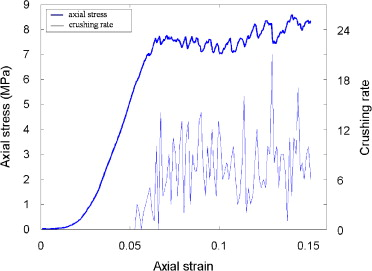
\includegraphics[width=\singleimagewidth]{chapters/figures/markets-bolton-stress-strain-crushing.jpg}
	\caption{Stress-strain response of a pebble bed with crushed pebbles. Reproduced from Ref.~\cite{Marketos2007}}
	\label{fig:marketos-bolton-stress-strain}
\end{figure}

\begin{figure}[!t]
\centering
	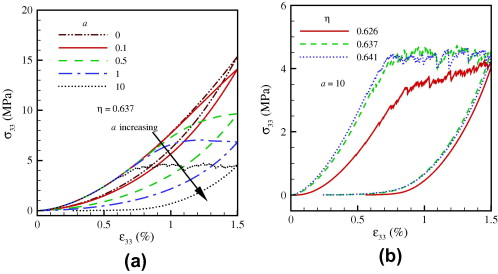
\includegraphics[width=\singleimagewidth]{chapters/figures/annabattula-stress-strain-crushing.jpg}
	\caption{Stress-strain response of a pebble bed with crushed pebbles. Reproduced from Ref.~\cite{Annabattula2012a}}
	\label{fig:annabattula-stress-strain}
\end{figure}

This numerical study will focus on the `what happens' question. In work by Marketos and Bolton, they treated a crushed pebble very similar to Van Lew\etal~; when a pebble was damaged it was removed completely from the assembly.\cite{Marketos2007,VanLew2014} Marketos and Bolton study the stress-strain response of a pebble bed with a predictive crushing routine while we studied the effective thermal conductivity of a damaged pebble bed.

However, the technique of removing a pebble is limited by the fact that energy input into two systems being studied is not comparable. Because we have volumetric energy deposition in our simulations, the total energy pouring into the non-damaged system would be
\begin{equation}
	E_h = \frac{q'''_\text{nuc} V_\text{peb} N}{V_\text{bed}}
\end{equation}
where $N$ is the total number of pebbles of volume $V_\text{peb}$ that exist in the pebble bed of volume $V_\text{bed}$. After a crushing event, when we remove pebbles, the total amount of energy is
\begin{equation}
	E_h' = \frac{q'''_\text{nuc} V_\text{peb} \eta N}{V_\text{bed}}
\end{equation}
where $\eta$ is the percent of crushed pebbles. Obviously then, the ratio of the two heating rates is\begin{equation}
	\frac{E_h'}{E_h} = 1 - \eta
\end{equation}
and the energy deposited is not balanced between a virgin bed and one with crushed pebbles. We will attempt to address this issue.

\subsection{Modeling a Crushed Pebble}
In the DEM framework, we are limited to modeling elastic spheres. If we strictly wish to conserve mass between a solid pebble of radius $R_p$ and the crushed fragments of radius $R_c$, then the number of crushed fragments (spheres) per crushed pebble is
\begin{equation}\label{eq:nc-crushed-fragments}
	N_c = \left(\frac{R_c}{R_p}\right)^{-3}
\end{equation}

Thus the number of fragments goes like the inverse of radius ratio to the third power and the number of crushed fragments to represent a single crushed pebble increases rapidly as the fragments shrink.


\begin {table}[htp] %
\caption{Example values of the particle crush fragments, $N_c$, necessary to replace a single crushed particle and obey conservation of mass (fragment number is rounded to nearest integer).}
\label {tab:rstar-Nc} \centering %
\begin {tabular}{ S[table-format=3.2]S[table-format=3.2] }
\toprule
$R_c/R_p$ 						& $N_c$  				\\\otoprule
0.20                            & 125                   \\    
0.30                            & 37               \\
0.40                            & 16                   \\
0.50                            & 8                         \\
0.75                            & 2                \\\bottomrule
\end{tabular}
\end{table}

The relationship between radius ratio and number of fragment particles is given in Fig.~\ref{fig:fragment-count}. Note that in the DEM simulation, it is impossible to insert fractions of a particle so the number of fragment pebbles is rounded to the nearest integer in the figure.

\begin{figure}[!t]
\centering
    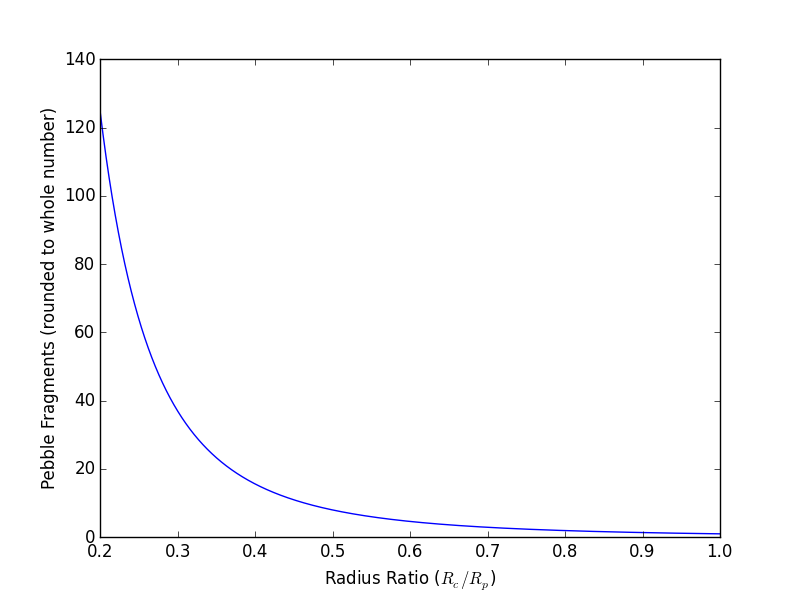
\includegraphics[width=\singleimagewidth]{chapters/figures/crush-fragments/pebble-fragment-count.png}
    \caption{Number of fragment pebbles necessary to conserve mass increases rapidly as the size of the radius ratio ($\frac{R_c}{R_p}$) decreases.}
    \label{fig:fragment-count}
\end{figure}

In typical DEM simulations that can run within reasonable amounts of time on the machines available to me in this dissertation, a reasonable number of particles is around 10~000. Many more and the run times become impractical for study. To show how quickly the number of particles can quickly get out of hand in a simulation, if we begin with 6~000 pebbles and only 2\% break, with a radius ratio of $R_c/R_p = 0.2$, the number of pebbles to be added would be 15~000. The new particle fragments (less the crushed particles) plus the original would require 21~000 particles in the system. In our simulations, we often test the effects on effective thermal conductivity at particle crush amounts of to 10\%. For the pebble bed mentioned here, that would mean 81~000 particles in the system and it would be computationally forbidding. The result is that, for computational times, the larger crush fragment radii are desired, \textit{i.e.} $R_c/R_p > 0.3$.

However, aside from satisfying conservation of mass, we must physically insert the particle fragments into void space in the simulation domain. During the course of the simulation, when we choose to replace the pebble with the fragments, the only available room is the spherical void left over by the damaged pebble. Other constraint is the smallest sized sphere that will allow the given spheres at most dense packing. 

Dense packing of spheres inside a larger sphere is an interesting mathematical problem. \href{http://www.randomwalk.de/sphere/insphr/spisbest.txt}{Hugh Pfoertner} keeps a compiled list of many solutions for a number of particles; many solutions are his are from Gensane.\cite{gensane2003dense}

If we consider, for instance, that a radius ratio of $R_c/R_p = 0.3$ requires 37 particle fragments, then we can also find from Ref.~\cite{gensane2003dense} that 37 particles would have to be of radius 0.2406866 to fit into a single sphere of radius of unity. We defined the particle fragment radius as $R_c$, the original particle as $R_p$, and then radius of sphere necessary to hold the $N_c$ fragments will be $R_N$, we can find a relationship between the volume of sphere $V_p$ and necessary volume $V_N$,
\begin{equation}
	r_1^* = \frac{R_c}{R_p}
\end{equation}
and
\begin{equation}
	r_2^* = \frac{R_c}{R_N}
\end{equation}
then 
\begin{equation}
	R_N = R_p \frac{r_1^*}{r_2^*}
\end{equation}
thus
\begin{equation}
	\frac{V_N}{V_p} = \left(\frac{r_1^*}{r_2^*}\right)^3
\end{equation}

If we choose a linearly spaced distribution of $r_1^*$ between 0 and 1, we can then find how many $N_c$ particles are necessary to conserve mass, then from the $N_c$ particles we can find from the database of sphere packing solutions the size of sphere that would be necessary to fit the $N_c$ particles. The calculations are carried out and shown in Fig.\ref{fig:volume-ratio}. The data in Ref.~\cite{gensane2003dense} does not go above 72 spheres so we are limited to radius ratios above about $r_1^* > 0.24$.

The plot shows that for particle fragments of reasonable numbers ($N_c\approx 20$ for $r_1^*\approx 0.3$), the volume necessary to fit the number of volume-conserving particles is greater than double the volume of the original sphere! 

\begin{figure}[!t]
\centering
    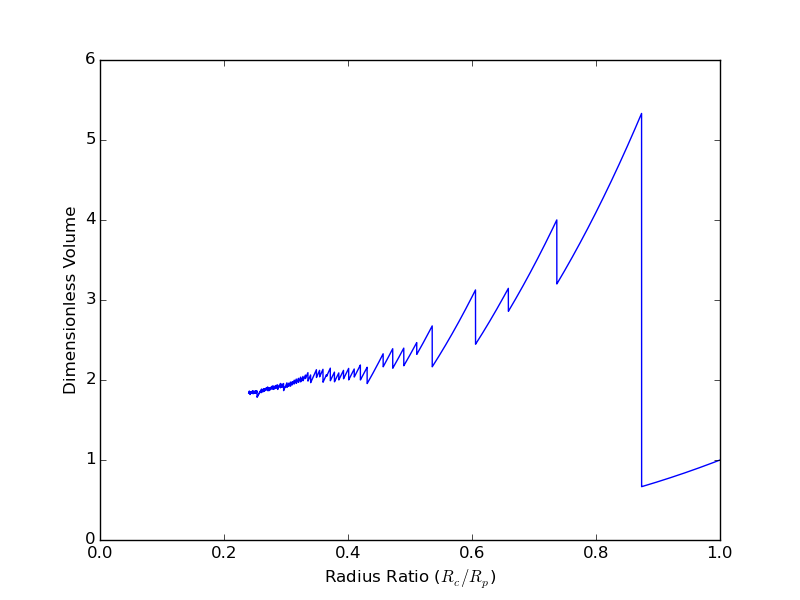
\includegraphics[width=\singleimagewidth]{chapters/figures/crush-fragments/fragment-volume-ratio.png}
    \caption{The volume necessary to house the particles of different radius ratios decreases toward unity as the radius ratio decreases. It is greater than 5 times the volume for large $r_1^*$.}
    \label{fig:volume-ratio}
\end{figure}

Therefore from the point of view of having the physical space to insert the fragments, smaller sized fragments is ideal. To insert the few number of large particles would require disrupting the packing in the region of the damaged particle.

Thus we have competing results from the two requirements. Computationally, we desire larger crushed fragments yet we need smaller fragments in order to fit them into the system in a non-disruptive way.


\begin{figure}[!ht]
	\centering
	\begin{subfigure}[b]{\doubleimagewidth}
		\centering
		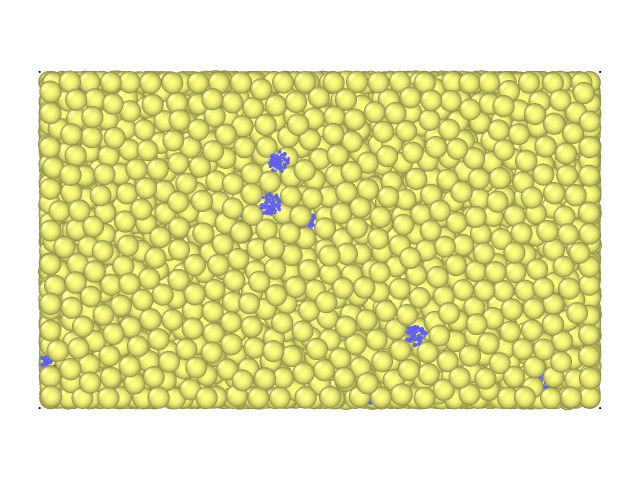
\includegraphics[width=\textwidth]{chapters/figures/crush-fragments/0.20-1.png}
		\caption{initial}
	\end{subfigure}
	\begin{subfigure}[b]{\doubleimagewidth}
		\centering
		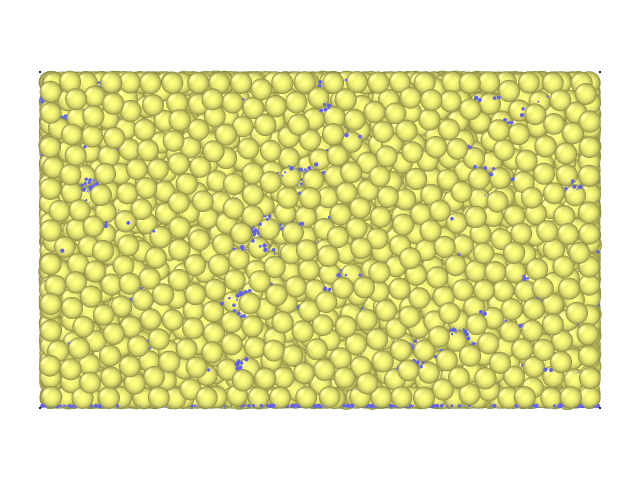
\includegraphics[width=\textwidth]{chapters/figures/crush-fragments/0.20-2.png}
		\caption{final}
	\end{subfigure}
	\caption{$N_c = 8594$, $N_\text{tot} = 15430$, $r_1^* = 0.20$. Side view of the packing arrangement and settling for different crush fragment sizes. The small crush fragments migrate far through the height of the bed. The yellow particles are the original pebbles and the blue are fragments inserted into the system after pebble crushing.}
\label{fig:crush-settling-pictures-1}
\end{figure}
\begin{figure}[!ht]
	\begin{subfigure}[b]{\doubleimagewidth}
		\centering
		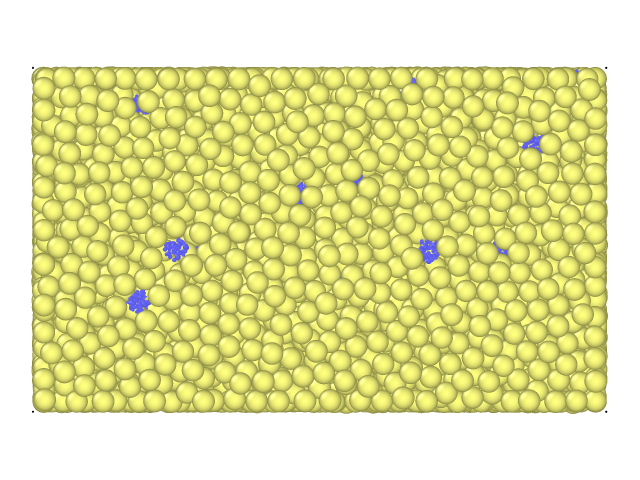
\includegraphics[width=\textwidth]{chapters/figures/crush-fragments/0.25-1.png}
		\caption{initial}
	\end{subfigure}
	\begin{subfigure}[b]{\doubleimagewidth}
		\centering
		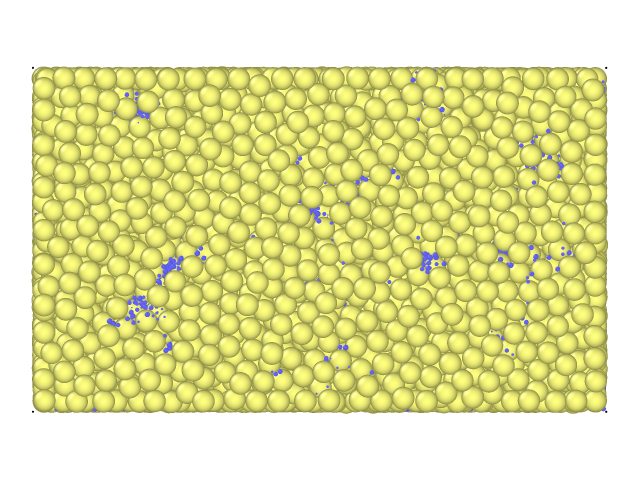
\includegraphics[width=\textwidth]{chapters/figures/crush-fragments/0.25-2.png}
		\caption{final}
	\end{subfigure}
	\caption{$N_c = 4400$, $N_\text{tot} = 11222$, $r_1^* = 0.25$. Side view of the packing arrangement and settling for different crush fragment sizes. The small crush fragments migrate far through the height of the bed. The yellow particles are the original pebbles and the blue are fragments inserted into the system after pebble crushing.}
\label{fig:crush-settling-pictures-2}
\end{figure}

\begin{figure}[!ht]
	\centering
	\begin{subfigure}[b]{\doubleimagewidth}
		\centering
		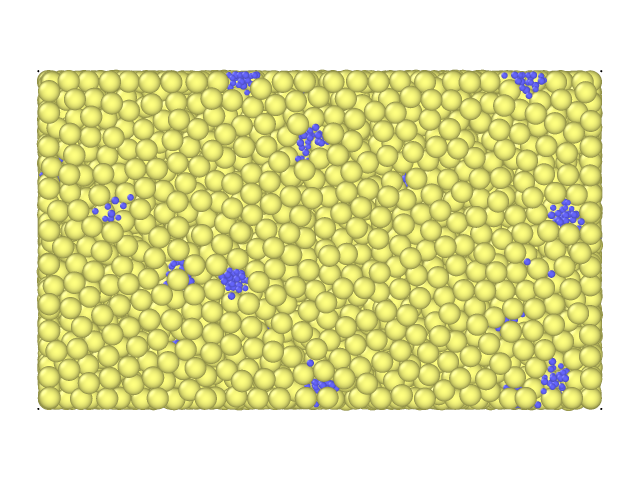
\includegraphics[width=\textwidth]{chapters/figures/crush-fragments/0.35-1.png}
		\caption{initial}
	\end{subfigure}
	\begin{subfigure}[b]{\doubleimagewidth}
		\centering
		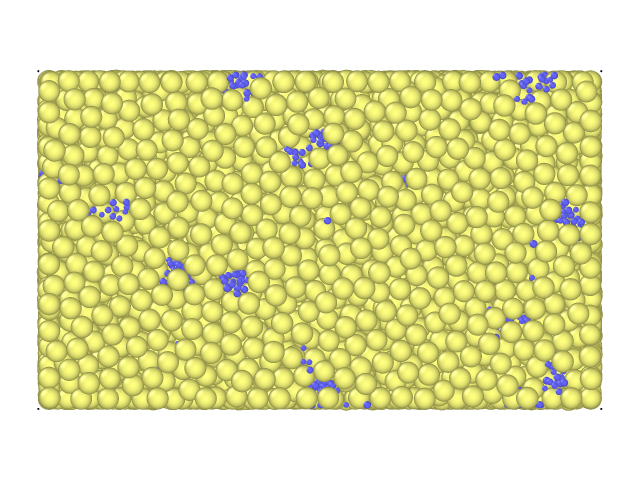
\includegraphics[width=\textwidth]{chapters/figures/crush-fragments/0.35-2.png}
		\caption{final}
	\end{subfigure}
	\caption{$N_c = 1603$, $N_\text{tot} = 8393$, $r_1^* = 0.35$. Side view of the packing arrangement and settling for different crush fragment sizes. The bigger fragments remain largely in place. The yellow particles are the original pebbles and the blue are fragments inserted into the system after pebble crushing.}
\label{fig:crush-settling-pictures-3}
\end{figure}
\begin{figure}[!ht]
	\begin{subfigure}[b]{\doubleimagewidth}
		\centering
		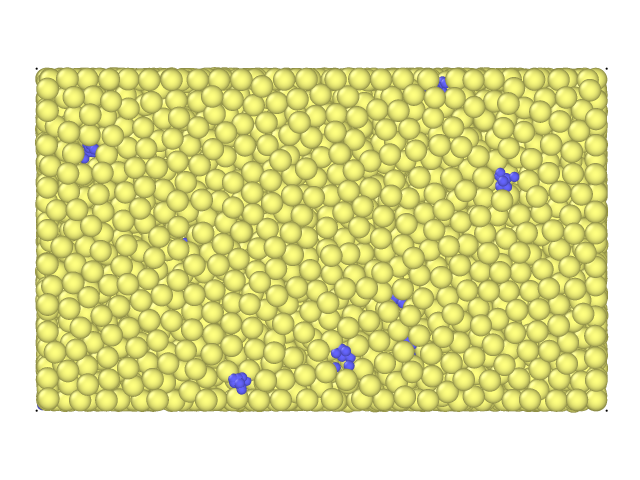
\includegraphics[width=\textwidth]{chapters/figures/crush-fragments/0.50-1.png}
		\caption{initial}
	\end{subfigure}
	\begin{subfigure}[b]{\doubleimagewidth}
		\centering
		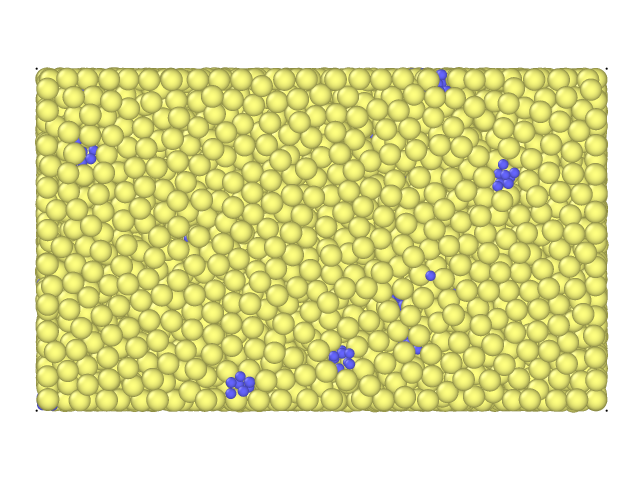
\includegraphics[width=\textwidth]{chapters/figures/crush-fragments/0.50-2.png}
		\caption{final}
	\end{subfigure}
	\caption{$N_c = 550$, $N_\text{tot} = 7358$, $r_1^* = 0.50$. Side view of the packing arrangement and settling for different crush fragment sizes. The bigger fragments remain largely in place. The yellow particles are the original pebbles and the blue are fragments inserted into the system after pebble crushing.}
\label{fig:crush-settling-pictures-4}
\end{figure}
\FloatBarrier

Lastly, in this packing study we look at the displacement of the particle fragments after insertion into the system and as they come to rest in a steady state. We began with 6~875 particles and randomly crushed 1\%. This was done with a range of fragments of size $r_1^* = [0.20, 0.25, 0.35, 0.50]$. The number of particles inserted followed the from Eq.~\ref{eq:nc-crushed-fragments}. In the images of Figs.~\ref{fig:crush-settling-pictures-1},~\ref{fig:crush-settling-pictures-2},~\ref{fig:crush-settling-pictures-3}, and~\ref{fig:crush-settling-pictures-4}, we see the initial packing of new particle fragments (in blue) settle into the interstitial gaps of the packing structure of original pebbles (yellow).

\begin{figure}[!t]
\centering
    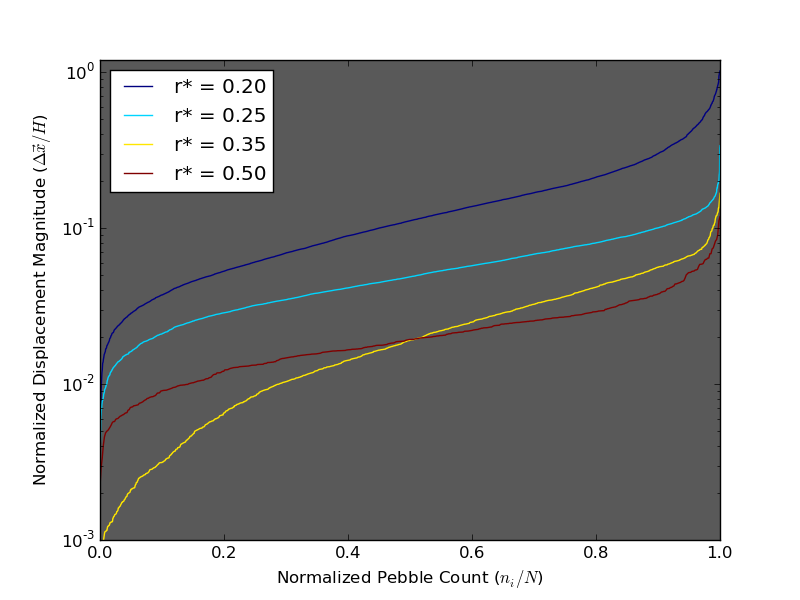
\includegraphics[width=\singleimagewidth]{chapters/figures/crush-fragments/displacement-scatter-radius-ratios.png}
    \caption{After the particle fragments are inserted into the system they re-settle due to gravity and inter-particle forces. The small fragments travel much further throughout the bed than the large fragments.}
    \label{fig:displacement-scatter}
\end{figure}

The settling of crushing fragments is also visualized in Fig.~\ref{fig:displacement-scatter}. In this figure, the magnitude of displacement for all the crushed fragments is recorded based on the change between initial insertion location and final resting place. The displacement of the fragments is normalized against the height of the pebble bed, $H$. The fragments with $r_1^* = 0.2$ are seen to travel, on average, 10\% of the height of the pebble bed before coming to rest; some of them travel more than the entire height of the bed! In contrast, the particle fragments of size $r_1^* = 0.35$ and $r_1^* = 0.5$ travel only about 1\% of the height of the bed before coming to rest. 

\begin{figure}[!t]
\centering
    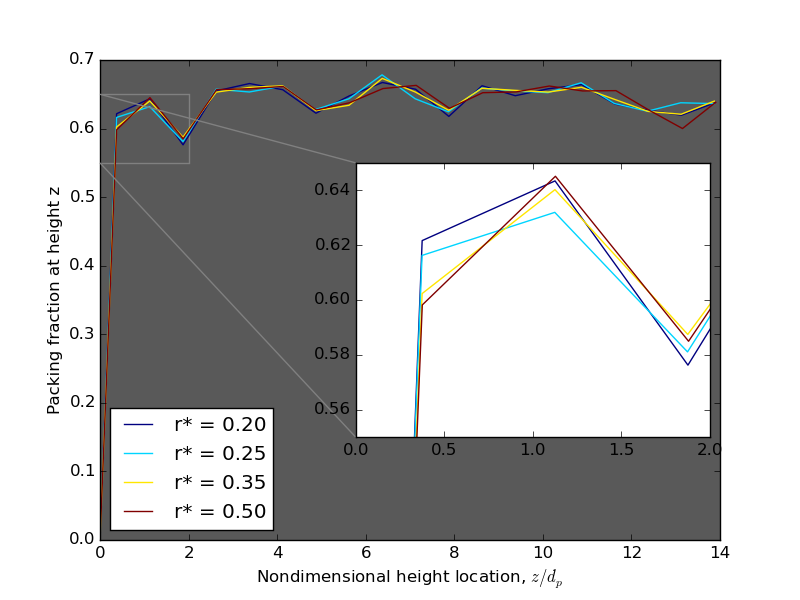
\includegraphics[width=\singleimagewidth]{chapters/figures/crush-fragments/packing-fraction-height.png}
    \caption{For only 1\% of crushed pebbles, the re-settling of small pebble fragments has a small effect on the overall packing fraction of the pebble bed. In the inset, the main influence is seen in the slight increase of packing fraction within the first pebble radius of the floor.}
    \label{fig:fragment-packing-fraction}
\end{figure}

From Fig.~\ref{fig:displacement-scatter}, the impression then arises that the large displacement magnitudes of the small crush fragments would result in an overall less-dense bed with large increase in packing fraction near the floor where pebbles settle. However, there is no observable changes to the local packing fraction along the height of the pebble bed. In Fig.~\ref{fig:fragment-packing-fraction}, the packing fraction of the four different pebble beds is given. We chose to only simulate a small percentage of crushed pebbles in these simulations. 